\chapter{Machine Learning Modeling Review}
\label{ch2}
This section first introduces the fundamentals of machine learning model training and testing, then details the fundamental architectures relevant to this work, and finally reviews the core components in model training: improvement from examples.

\section{Fundamentals of Model Training and Testing}
Figure \ref{fig:simple_model_training} is a simple diagram of how a machine learning model iteratively improves from examples, a process called ``training" or ``learning." Inputs and weights are sent into the model which applies the weights to the inputs to produce a result. The result is analyzed for performance, and based on the performance an update is applied to the weights which will improve model performance.
\begin{figure}[h!]
	\centering
		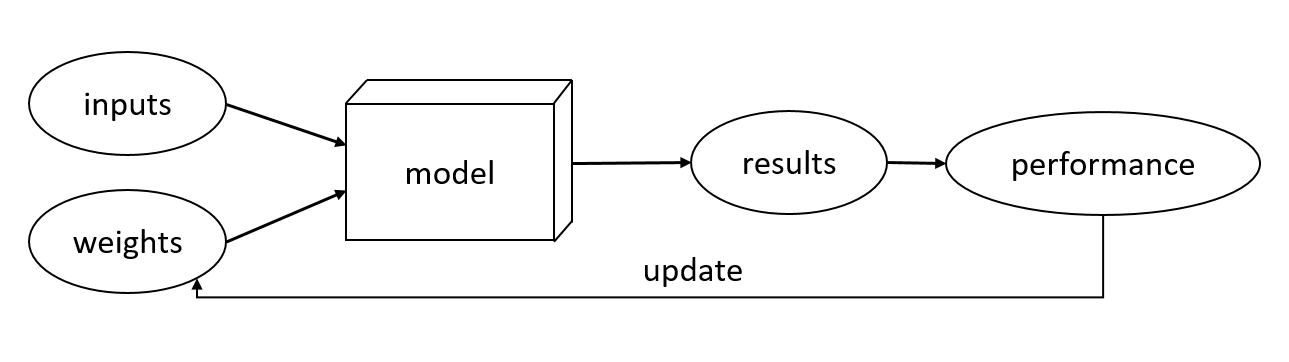
\includegraphics[width=0.99\textwidth]
		{training_process.png}
		\hfill
		\caption{Simple example of machine learning model training .}
		\label{fig:simple_model_training}
\end{figure}
This process is done iteratively until model performance stops improving, i.e., the model has converged to a solution. The final set of weights are the model's trained, or learned, parameters. The modeling described is an example of ``supervised learning" in which a set of inputs is associated with a known (truth) value trying to be modeled. The performance analysis compares the model output with the truth value.

The trained model is then ready for testing, or inference, on another set of inputs. Figure \ref{fig:simple_model_testing} illustrates this process.
\begin{figure}[h!]
	\centering
	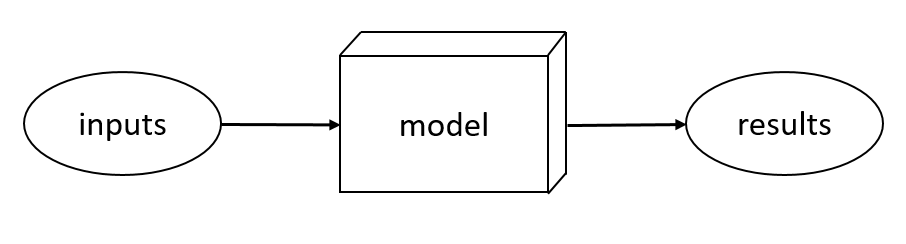
\includegraphics[width=0.99\textwidth]
	{testing_process.png}
	\hfill
	\caption{Simple example of machine learning model testing.}
	\label{fig:simple_model_testing}
\end{figure}
The learned parameters from the training process are static in the model and are applied to the inputs to produce a result. The test inputs must be in the same format of the inputs used during training. While not required, it's highly desirable for the test inputs to be of similar magnitudes as the train inputs.

\section{Machine Learning Model Architectures}
\label{sec:architectures}
The section reviews the fundamental architectures explored in this work: the Multilayer Perceptron and the Recurrent Neural Network. Additionally presented is a brief overview of how a model processes from input to output.

\subsection{Multilayer Perceptron}
The \ac{MLP} is a feedforward \ac{ANN} consisting of at least three layers of nodes: an input layer, a hidden layer, and an output layer. The number of hidden layers in an \ac{MLP} is adjustable to be greater than one. Each node in the \ac{MLP} is a value, also called the node's activation. Each node in the input layer represents an input variable. Each node in the hidden and output layers represent the weighted sum of the activations from the previous layer. The \ac{MLP} is described as ``fully-connected" because each node in one layer connects with a specific weight $w_{ij}$ to every node in the following layer.

Figure \ref{fig:architecture_MLP_simple} is a simple 2-layer \ac{MLP} for turbulence ($C_{n}^{2}$) modeling. The input layer, which is not counted towards the depth (number of layers) of the \ac{NN}, is five nodes wide. Each input node represents a weather variable measurement: temperature, pressure, relative humidity, wind speed, and solar irradiance.
\begin{figure}[h!]
	\centering
	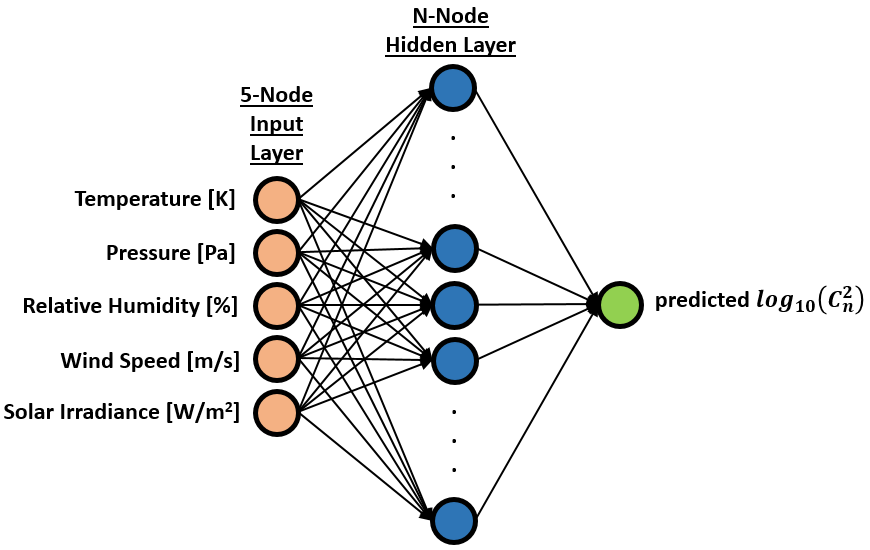
\includegraphics[width=0.99\textwidth]
	{architecture_MLP_simple.png}
	\hfill
	\caption{Simple MLP (multi-layer perceptron) to predict $log_{10}(C_{n}^{2})$ from weather inputs.}
	\label{fig:architecture_MLP_simple}
\end{figure}
The input layer is fully-connected to the only hidden layer which is N-nodes wide. In application the researcher sets N. The hidden layer is described as ``hidden" because its nodes are buried in the model, i.e., are not part of the \emph{inputs} or the \emph{outputs}. The arrows from input layer to hidden layer in Figure \ref{fig:architecture_MLP_simple} illustrate the concept of an \ac{MLP} being fully-connected: an arrow points from each node in the input layer to each node in the hidden layer. This is further shown in the full connection between the hidden layer and output layer which has only a single node. The \ac{NN} in Figure \ref{fig:architecture_MLP_simple} is a single-output \emph{regression} \ac{MLP} because the output layer is a single node of \emph{continuous} values. Specifically, the \ac{MLP} in Figure \ref{fig:architecture_MLP_simple} models the relationship between a set of weather inputs and $log_{10}{C_{n}^{2}}$ value. The other major \ac{NN} type is \emph{classification} which predicts/classifies \emph{discrete} values or labels. Only regression \ac{NN} is used in this work.

When fully-connected, the activations of a layer of nodes are calculated from the prior layer's node activations by
\begin{equation} \label{eq:MLP}
	\vec{y} = \sigma \left(\textbf{W}\vec{x} + \vec{b}\right)
\end{equation}
where $\vec{x}$ is the input vector of prior layer node activations, $\vec{y}$ is the output vector of next layer node activations, $\textbf{W}$ and $\vec{b}$ are the learnable matrix weights and vector biases, and $\sigma$ is a non-linear activation function. In matrix notation, Equation \ref{eq:MLP} for a 2-node layer fully-connected to another 2-node layer is written
\begin{equation} \label{eq:MLP_matrix}
	\begin{bmatrix}
		y_{1} \\
		y_{2}
	\end{bmatrix}
	= \sigma \left(
	\begin{bmatrix}
		w_{1,1} & w_{1,2} \\
		w_{2,1} & w_{2,2}
	\end{bmatrix}
	\begin{bmatrix}
		x_{1} \\
		x_{2}
	\end{bmatrix}
	+
	\begin{bmatrix}
		b_{1} \\
		b_{2}
	\end{bmatrix}
	\right).
\end{equation}
The matrix-vector product $\textbf{W}\vec{x}$ is the weighted sum of the learnable weights and the input layer node activations. The notation of the weight matrix elements $w_{ij}$ is such that $i$ is the $i^{th}$ node of the output layer and $j$ is the $j^{th}$ node of the input layer. The elements in the bias vector $\vec{b}$ are similar to the constant $b$ of a linear function
\[
y = ax + b
\]
that allows the model to best fit for the given data. The size of the learnable weight matrix ($\textbf{W}$) is $\left[\text{output size} \times \text{input size}\right]$, and the size of the learnable bias vector ($\vec{b}$) is $\left[\text{output size}\right]$. ``Input size" is the number of nodes in the first layer, and ``output size" is the number of nodes in the second layer.

The matrix-vector product of the weights and inputs and the addition of the bias vector are purely linear which constrains the model to learn only linear relationships. The $\sigma$ in Equations \ref{eq:MLP} and \ref{eq:MLP_matrix} is a non-linear activation function applied element-wise to the values calculated from 
\[
\begin{bmatrix}
	w_{1,1} & w_{1,2} \\
	w_{2,1} & w_{2,2}
\end{bmatrix}
\begin{bmatrix}
	x_{1} \\
	x_{2}
\end{bmatrix}
+
\begin{bmatrix}
	b_{1} \\
	b_{2}
\end{bmatrix}
\]
to allow the model to learn non-linear relationships. The particular non-linear activation function $\sigma$ is the sigmoid which squishes its argument between 0 (zero) and 1 by
\begin{equation} \label{eq:sigmoid}
	\text{sigmoid}\left(x\right) = \sigma \left(x\right) = \frac{1}{1 + \exp \left(-x\right)}.
\end{equation}
Figure \ref{fig:activation_functions_a} \cite{PyTorch} illustrates the effect of the sigmoid activation function. Two additional activation functions used in this work are the hyperbolic tangent ($\tanh$) defined as
\begin{equation} \label{eq:tanh}
	\tanh \left(x\right) = \frac{\exp \left(x\right) - \exp \left(-x\right)}{\exp \left(x\right) + \exp \left(-x\right)},
\end{equation}
and the \ac{ReLU} defined as
\begin{equation} \label{eq:relu}
	\text{ReLU} \left(x\right) = \max \left(0, x\right).
\end{equation}
The $\tanh$ is similar to the sigmoid but is a smoother zero-centered activation function whose range lies between -1 and +1 as illustrated in Figure \ref{fig:activation_functions_b}. The \ac{ReLU} is a piecewise linear function that returns a positive input as itself but returns 0 (zero) if the input is negative as shown in Figure \ref{fig:activation_functions_c}. The nearly linear \ac{ReLU} preserves the properties of linear models that make them easy to optimize with gradient descent methods. The \ac{RNN} architectures explored in this work use the sigmoid and $\tanh$ activation functions, and the \ac{MLP} architectures use the ReLU which is the most commonly used activation function in deep learning models. Details on the advantages and disadvantages of these activation functions are explored by Nwankpa \cite{activationfunctions}.
\begin{figure}[p!]
 	\centering
 	\subfloat[Telescope setup\label{fig:activation_functions_a}]{
 		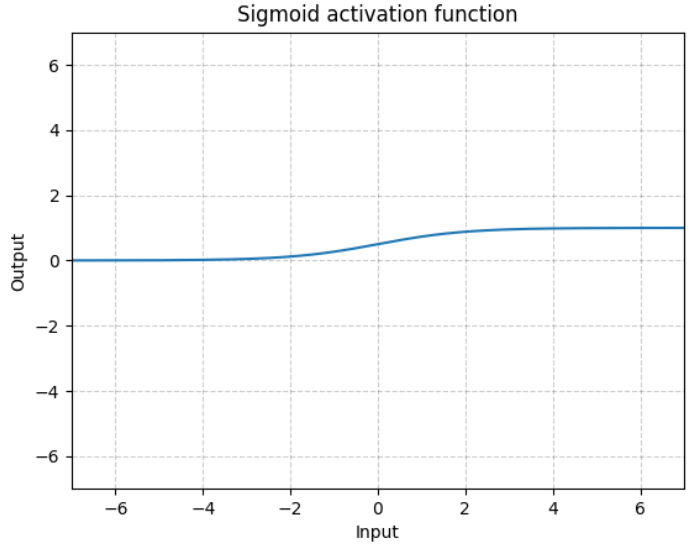
\includegraphics[width=0.49\textwidth]
 		{activation_function_Sigmoid.png}
 	}
 	\hfill
 	\subfloat[Telescope setup\label{fig:activation_functions_b}]{
 		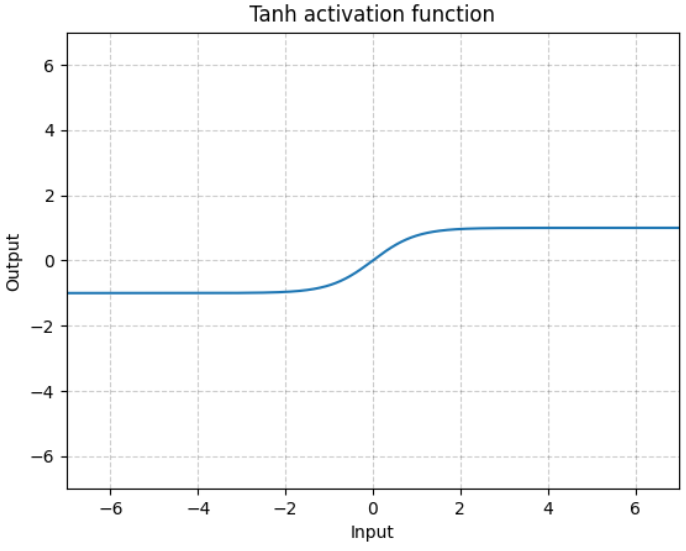
\includegraphics[width=0.485\textwidth]
 		{activation_function_tanh.png}
 	}
 	\subfloat[Wide view of target\label{fig:activation_functions_c}]{
 		\includegraphics[width=0.49\textwidth]
 		{activation_function_ReLU.png}
 	}
 	\hfill
 	\caption{Sigmoid ($\sigma$), hyperbolic tangent ($\tanh$), and Rectified Linear Unit (ReLU) activation functions.}
 	\label{fig:activation_functions}
\end{figure}

\subsection{Recurrent Neural Networks}
A \ac{RNN} is an extension of a conventional feedforward neural network which is able to handle a variable-length sequence input. The \ac{RNN} handles the variable-length sequence by having a recurrent hidden state whose activation (value) at each time is dependent on that of the previous time \cite{GRU}. This processing is illustrated in Figure \ref{fig:architecture_RNN_single_layer_unrolled} where $x_{t}$ is the set of inputs at time $t$ and $h_{t}$ is the resulting hidden state at time $t$. The left side of Figure \ref{fig:architecture_RNN_single_layer_unrolled} is the rolled version of the \ac{RNN} processing and the right side is the unrolled version.
\begin{figure}[h!]
	\centering
	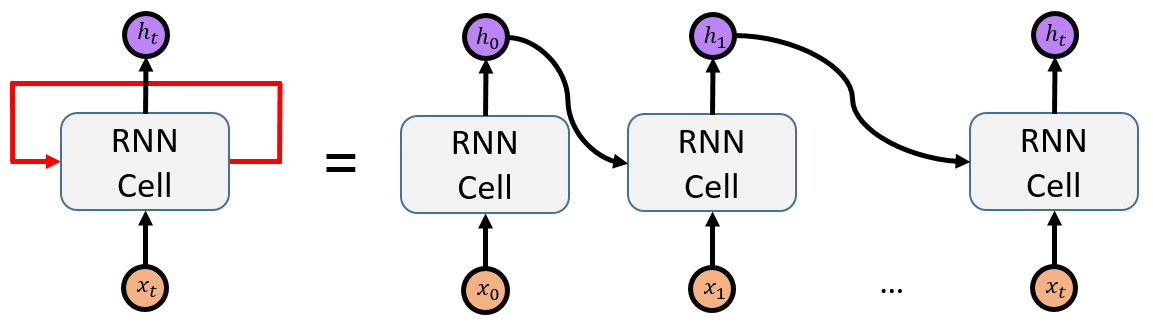
\includegraphics[width=0.99\textwidth]
	{architecture_RNN_single_layer_unrolled.png}
	\hfill
	\caption{Unrolled single-layer RNN}
	\label{fig:architecture_RNN_single_layer_unrolled}
\end{figure}
At time $t=0$ the inputs are fed into the \ac{RNN} cell which calculates hidden state $h_{0}$. This hidden state is then fed into the \ac{RNN} cell in combination with the inputs at time $t=1$ to calculate the hidden state $h_{1}$. This process continues until the final input of the time series $x_{t}$ is sent into the \ac{RNN} cell with hidden state $h_{\left(t-1\right)}$ to calculate the final hidden state $h_{t}$ which can be the model output or further manipulated in a more complex architecture. The internal processing of the \ac{RNN} cell is discussed later.

The architecture in Figure \ref{fig:architecture_RNN_single_layer_unrolled} is a single-layer \ac{RNN} that behaves similarly to the \ac{MLP} in Figure \ref{fig:architecture_MLP_simple} which has only a single hidden layer. More hidden layers are needed to add complexity (depth) to the \ac{NN}. Additional hidden layers in a \ac{RNN} look like Figure \ref{fig:architecture_RNN_multi_layer_unrolled}. Like the single-layer \ac{RNN}, the first layer of the multi-layer \ac{RNN} processes prior hidden state $h_{\left(t-1\right)}$ and and current input $x_{t}$ to hidden state $h_{t}$.
\begin{figure}[h!]
	\centering
	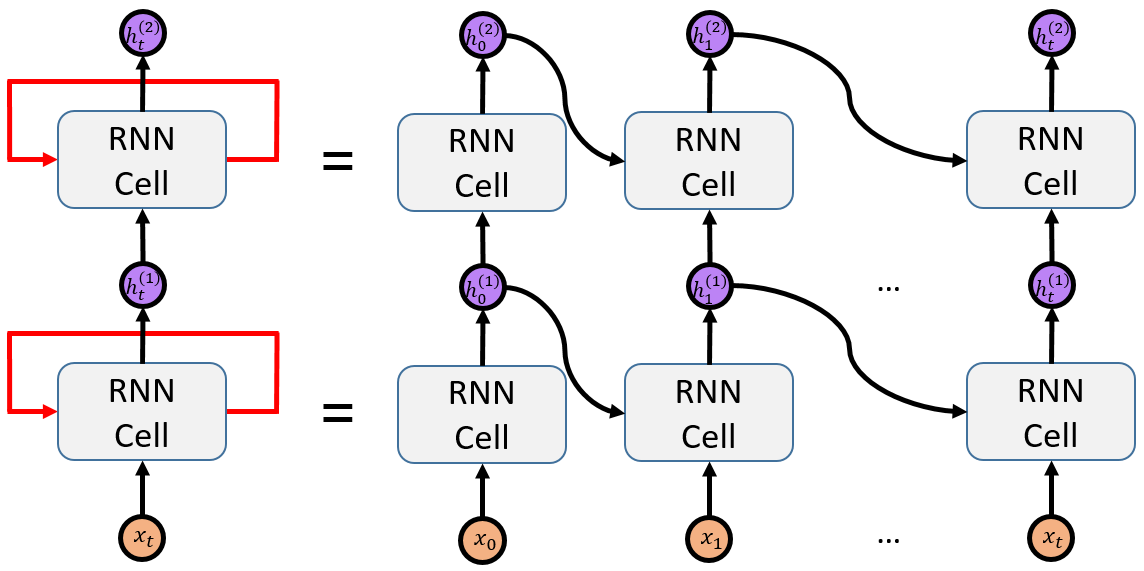
\includegraphics[width=0.99\textwidth]
	{architecture_RNN_multi_layer_unrolled.png}
	\hfill
	\caption{Unrolled multi-layer RNN}
	\label{fig:architecture_RNN_multi_layer_unrolled}
\end{figure}
After the inputs from each step are processed the result is sent to the next layer. In this layer the processing is done in the exact same fashion but the inputs are now the hidden state at each time $h_{t}$ from the prior layer instead of the input variables $x_{t}$. In the left of Figure \ref{fig:architecture_RNN_multi_layer_unrolled} is the rolled version of the multi-layer \ac{RNN} which shows $x_{t}$ being repeatedly processed by the \ac{RNN} cell to $h_{t}^{(1)}$ which is the first-layer hidden state. $h_{t}^{(1)}$ is then the input to the second layer \ac{RNN} which processes the data to second-layer hidden state $h_{t}^{(2)}$. The right of Figure \ref{fig:architecture_RNN_multi_layer_unrolled} is the unrolled version which further illustrates the multi-layer \ac{RNN} processing.

\section{Recurrent Neural Network Cells}
There are many variants of the \ac{RNN} cells in Figures \ref{fig:architecture_RNN_single_layer_unrolled} and \ref{fig:architecture_RNN_multi_layer_unrolled} that process each time step of the input sequence. This thesis explores three of the cell variants: the simple (original) \ac{RNN}, the \ac{LSTM-RNN}, and the \ac{GRU-RNN}. The \ac{LSTM-RNN} and \ac{GRU-RNN} are two of the most widely used \ac{RNN} cell variants.

\subsection{Simple RNN}
At each time step $t$ the hidden state $\vec{h}_{t}$ of the simple \ac{RNN} is updated by
\begin{equation} \label{eq:RNN}
	\vec{h}_{t} = \tanh\left(\textbf{W}_{ih} \vec{x}_{t} + \vec{b}_{ih} + \textbf{W}_{hh} \vec{h}_{\left(t-1\right)} + \vec{b}_{hh}\right)
\end{equation}
where $\tanh$ is the activation function that bounds the outputs from -1 to +1, $\vec{x}_{t}$ is the input at time $t$, $\vec{h}_{\left(t-1\right)}$ is the hidden state of the previous layer at time $t-1$ or the initial state at time 0 (zero), $\textbf{W}_{ih}$ is the learnable input-hidden weights, $\vec{b}_{ih}$ is the learnable input-hidden bias, $\textbf{W}_{hh}$ is the learnable hidden-hidden weights, and $\vec{b}_{hh}$ is the learnable hidden-hidden bias. These learnable parameters are described as ``shared through time" because the same parameters are applied to the inputs regardless of the time step of the input time series. Equation \ref{eq:RNN} and upcoming \ac{LSTM-RNN} and \ac{GRU-RNN} equations are PyTorch implementations \cite{PyTorch}.

According to PyTorch, the size of the learnable parameters goes as follows. The learnable input-hidden weights ($\textbf{W}_{ih}$) are size $\left[\text{hidden size} \times \text{input size}\right]$ for the single-layer \ac{RNN} or first layer of the stacked \ac{RNN}. The input-hidden weights are of size $\left[\text{hidden size} \times \text{hidden size}\right]$ for the subsequent layers of the stacked \ac{RNN}. The learnable hidden-hidden weights ($\textbf{W}_{hh}$) are size $\left[\text{hidden size} \times \text{hidden size}\right]$ for each layer of the \ac{RNN}. The learnable input-hidden bias ($\vec{b}_{ih}$) of each layer is size $\left[\text{hidden size}\right]$, and the learnable hidden-hidden bias ($\vec{b}_{hh}$) of each layer is size $\left[\text{hidden size}\right]$. Note that ``input size" is the number of features (variables) in the input vector, and ``hidden size" is the number of hidden nodes per \ac{RNN} layer.

One significant issue with the simple \ac{RNN} is its struggle to capture long-term dependencies because the gradients tend to either vanish or explode. Training an \ac{RNN} with gradient-based optimization methods is a challenge because of the variations in gradient magnitudes and because the long-term dependencies are hidden by the effect of short-term dependencies \cite{GRU}. The other variants explored in this work are designed to handle this vanishing/exploding gradient problem.

\subsection{LSTM-RNN}
The \ac{LSTM-RNN} \cite{LSTM} deals with the vanishing/exploding gradient problem by proposing a new architecture and gradient-based learning algorithm. The \ac{LSTM-RNN} can learn to bridge time intervals in excess of 1000 steps by utilizing a constant (neither vanishing nor exploding) error flow throughout the architecture. The core idea behind the \ac{LSTM-RNN} is its \emph{cell state} whose size is the number of hidden \ac{LSTM-RNN} nodes specified by the researcher. The architecture removes or adds information to the cell state by the use of \emph{gates}.

The first step in the \ac{LSTM-RNN} is the forget gate $\vec{f}_{t}$ which decides what information is thrown away or ``forgotten" from the cell state. It combines the prior hidden state $\vec{h}_{t-1}$ and the current input $\vec{x}_{t}$ with learnable weights and biases $\textbf{W}_{if}$, $\textbf{W}_{hf}$, $\vec{b}_{if}$, and $\vec{b}_{hf}$ in
\begin{equation} \label{eq:LSTM_forget_gate}
	\vec{f}_{t} = \sigma\left(\textbf{W}_{if} \vec{x}_{t} + \vec{b}_{if} + \textbf{W}_{hf} \vec{h}_{\left(t-1\right)} + \vec{b}_{hf}\right).
\end{equation}
The non-linear activation function is the sigmoid which squishes the values inside from 0 (zero) to 1. An output of 1 indicates to completely keep the prior information and an output of 0 (zero) indicates to completely remove the prior information.

The next step in the \ac{LSTM-RNN} combines the input gate $\vec{i}_{t}$ and cell gate $\vec{g}_{t}$ to determine what new information is passed into the cell state. The calculation of these gates is 
\begin{align}
\vec{i}_{t} &= \sigma\left(\textbf{W}_{ii} \vec{x}_{t} + \vec{b}_{ii} + \textbf{W}_{hi} \vec{h}_{\left(t-1\right)} + \vec{b}_{hi}\right) \label{eq:LSTM_input_gate} \\
\vec{g}_{t} &= \tanh\left(\textbf{W}_{ig} \vec{x}_{t} + \vec{b}_{ig} + \textbf{W}_{hg} \vec{h}_{\left(t-1\right)} + \vec{b}_{hg}\right), \label{eq:LSTM_cell_gate}
\end{align}
where $\textbf{W}_{ii}$, $\textbf{W}_{hi}$, $\textbf{W}_{ig}$, and $\textbf{W}_{hg}$ are the learnable weights and $\vec{b}_{ii}$, $\vec{b}_{hi}$, $\vec{b}_{ig}$, and $\vec{b}_{hg}$ are the learnable biases. Like the forget gate, these learnable weights and biases are applied to the inputs $\vec{x}_{t}$ and prior hidden state $\vec{h}_{\left(t-1\right)}$. The $\sigma$ activation function around the input gate $\vec{i}_{t}$ decides how much to update the cell state where a value of 1 indicates to completely update the cell state and a value of 0 does not update at all. The $\tanh$ activation around the cell gate $\vec{g}_{t}$ squishes the values between -1 and +1 to be the new candidate node activations \cite{olah}.

The input gate $\vec{i}_{t}$ controls how much of the candidate node activations from cell gate $\vec{g}_{t}$ are passed into the cell state $C_{t}$ by
\begin{equation} \label{eq:LSTM_update_cell_state}
	\vec{C}_{t} = \vec{f}_{t} \odot \vec{C}_{\left(t-1\right)} + \vec{i}_{t} \odot \vec{g}_{t},
\end{equation}
where $\vec{f}_{t}$ is the forget gate that controls how much information is kept from the prior cell state $\vec{C}_{\left(t-1\right)}$, and $\odot$ is element-wise multiplication. As an example, if the \ac{LSTM-RNN} calculated to keep 25\% of the prior cell state and update with 50\% of the new candidate activations then Equation \ref{eq:LSTM_update_cell_state} would update the cell state by
\[
\vec{C}_{t} = 0.25 \odot \vec{C}_{\left(t-1\right)} + 0.50 \odot \vec{g}_{t}.
\]

The final calculation in the \ac{LSTM-RNN} updates the hidden state $\vec{h}_{t}$ by combining the updated cell state $C_{t}$ with the output gate $\vec{o}_{t}$ by
\begin{align}
\vec{o}_{t} &= \sigma\left(\textbf{W}_{io} \vec{x}_{t} + \vec{b}_{io} + \textbf{W}_{ho} \vec{h}_{\left(t-1\right)} + \vec{b}_{ho}\right) \label{eq:LSTM_output_gate} \\
\vec{h}_{t} &= \vec{o}_{t} \odot \tanh\left(\vec{C}_{t}\right), \label{eq:LSTM_updated_hidden_state}
\end{align}
where $\textbf{W}_{io}$ and $\textbf{W}_{ho}$ are the learnable weights, and $\vec{b}_{io}$ and $\vec{b}_{ho}$ are the learnable biases. The output gate combines these learnable parameters with the input $\vec{x}_{t}$ and prior hidden state $\vec{h}_{\left(t-1\right)}$ then squishes them from 0 (zero) to 1 with the $\sigma$ activation function. This gate controls how much of the updated cell state $\vec{C}_{t}$ (squished between -1 and +1 with the $\tanh$) is passed to the updated hidden state $\vec{h}_{t}$. A value of 0 (zero) for the output gate passes none of the cell state and a value of 1 passes everything from the cell state to the updated hidden state.

The calculations outlined in this section are performed in every step of the input time series. Like in the simple \ac{RNN}, the learnable weights and biases are shared through time, i.e., they do not change between hidden state updates. According to PyTorch \cite{PyTorch} the number of learnable parameters goes as follows. The learnable input-hidden weights ($\textbf{W}_{ii}$, $\textbf{W}_{if}$, $\textbf{W}_{ig}$, $\textbf{W}_{io}$) are of size $\left[\text{4} \times \text{hidden size} \times \text{input size}\right]$ in the first \ac{LSTM-RNN} layer and $\left[\text{4} \times \text{hidden size} \times \text{hidden size}\right]$ in subsequent layers of a stacked \ac{LSTM-RNN}. The learnable hidden-hidden weights ($\textbf{W}_{hi}$, $\textbf{W}_{hf}$, $\textbf{W}_{hg}$, $\textbf{W}_{ho}$) are of size $\left[4 \times \text{hidden size} \times \text{hidden size}\right]$ in each layer of the \ac{LSTM-RNN}. The learnable input-hidden bias of each \ac{LSTM-RNN} layer ($\vec{b}_{ii}$, $\vec{b}_{if}$, $\vec{b}_{ig}$, $\vec{b}_{io}$) are size $\left[4 \times \text{hidden size}\right]$, and the learnable hidden-hidden bias of each \ac{LSTM-RNN} layer ($\vec{b}_{hi}$, $\vec{b}_{hf}$, $\vec{b}_{hg}$, $\vec{b}_{ho}$) are also size $\left[4 \times \text{hidden size}\right]$. Note that the multiplication by 4 does not apply to each weight or bias, but rather accounts for the combined size of all the biases. So for example bias $\vec{b}_{hi}$ is of size $\left[\text{hidden size}\right]$, but all four hidden-hidden biases are combined size $\left[4 \times \text{hidden size}\right]$. ``Hidden size" in this context is the number of hidden nodes in the \ac{LSTM-RNN} layer, and ``input size" is the number of features (variables) of the input vector.

\subsection{GRU-RNN}
The last variant of the \ac{RNN} cell is the \ac{GRU-RNN} that is motivated by the \ac{LSTM-RNN} but is much simpler to compute and implement \cite{GRU_original}. Instead of incorporating a cell state like the \ac{LSTM-RNN}, this cell architecture only applies updates to the hidden state. There are three gates in the \ac{GRU-RNN} architecture that are more general than the \ac{LSTM-RNN} gates: the reset gate $\vec{r}_{t}$, update gate $\vec{z}_{t}$, and the new gate $\vec{n}_{t}$.

The first calculation in the hidden state update for a single time step is the reset gate $r_{t}$ computed by
\begin{equation} \label{eq:GRU_reset_gate}
	\vec{r}_{t} = \sigma\left(\textbf{W}_{ir} \vec{x}_{t} + \vec{b}_{ir} + \textbf{W}_{hr} \vec{h}_{\left(t-1\right)} + \vec{b}_{hr}\right),
\end{equation}
where $\sigma$ is the sigmoid activation function, and $\vec{x}_{t}$ and $\vec{h}_{t-1}$ are the input and previous hidden state, respectively. $\textbf{W}_{ir}$ and $\textbf{W}_{hr}$ are the learnable input and hidden weight matrices, and $\vec{b}_{ir}$ and $\vec{b}_{hr}$ are the learnable input and hidden bias vectors.

Next, the update gate is computed by
\begin{equation} \label{eq:GRU_update_gate}
	\vec{z}_{t} = \sigma\left(\textbf{W}_{iz} \vec{x}_{t} + \vec{b}_{iz} + \textbf{W}_{hz} \vec{h}_{\left(t-1\right)} + \vec{b}_{hz}\right),
\end{equation}
where $\sigma$ is again the sigmoid activation function, and $\vec{x}_{t}$ and $\vec{h}_{t-1}$ are the input and previous hidden state, respectively. $\textbf{W}_{iz}$ and $\textbf{W}_{hz}$ are again the learnable input and hidden weight matrices, and $\vec{b}_{iz}$ and $\vec{b}_{hz}$ are the learnable input and hidden biases.

The proposed new hidden state is computed by
\begin{equation} \label{eq:GRU_new_gate}
		\vec{n}_{t} = \tanh\left(\textbf{W}_{in} \vec{x}_{t} + \vec{b}_{in} + \vec{r}_{t} \odot \left(\textbf{W}_{hn} \vec{h}_{\left(t-1\right)} + \vec{b}_{hn}\right)\right),
\end{equation}
where $\tanh$ is the activation function to range the values between -1 and +1, and $\vec{x}_{t}$ and $\vec{h}_{t-1}$ are the input and previous hidden state, respectively. $\textbf{W}_{in}$ and $\textbf{W}_{hn}$ are the learnable input and hidden weights, and $\vec{b}_{in}$ and $\vec{b}_{hn}$ are the learnable input and hidden biases. $\vec{r}_{t}$ is the reset gate from Equation \ref{eq:GRU_reset_gate}, and $\odot$ is element-wise multiplication.

The hidden state passed through the cell is computed by
\begin{equation} \label{eq:GRU_new_hidden_state}
	\vec{h}_{t} = \left(1 - \vec{z}_{t}\right) \odot \vec{n}_{t} + \vec{z}_{t} \odot \vec{h}_{\left(t-1\right)},
\end{equation}
where $\vec{z}_{t}$ is the update gate , $\vec{n}_{t}$ is the new gate, $\vec{h}_{t-1}$ is the previous hidden state, and $\odot$ is the element-wise multiplication.

When the reset gate $\vec{r}_{t}$ is close to 0 (zero), the hidden state is forced to ignore the previous hidden state and reset with the current input only. This effectively allows the hidden state to drop any information found to be irrelevant in the future. The update gate $\vec{z}_{j}$ controls how much information from the previous hidden state carries over to the current hidden state and helps the network remember long-term information. Each node in the hidden \ac{GRU-RNN} cell has separate reset and update gates, so each node learns to capture dependencies over different time scales. The nodes that learn short-term dependencies tend to have reset gates that are frequently active, but nodes that capture longer-term dependencies have update gates that are mostly active \cite{GRU_original}.

According to PyTorch \cite{PyTorch} the number of learnable parameters goes as follows. The learnable input-hidden weights ($\textbf{W}_{ir}$, $\textbf{W}_{iz}$, $\textbf{W}_{in}$) are of size $\left[3 \times \text{hidden size} \times \text{input size}\right]$ for the first layer and $\left[3 \times \text{hidden size} \times \text{hidden size}\right]$ for subsequent layers in the stacked \ac{GRU-RNN}. The learnable hidden-hidden weights ($\textbf{W}_{hr}$, $\textbf{W}_{hz}$, $\textbf{W}_{hn}$) in each layer are of size $\left[3 \times \text{hidden size} \times \text{hidden size}\right]$. The learnable input-hidden bias ($\vec{b}_{ir}$, $\vec{b}_{iz}$, $\vec{b}_{in}$) of each layer are size $\left[3 \times \text{hidden size}\right]$, and the learnable hidden-hidden bias ($\vec{b}_{hr}$, $\vec{b}_{hz}$, $\vec{b}_{hn}$) of each layer are size $\left[3 \times \text{hidden size}\right]$. Like described for the \ac{LSTM-RNN}, the multiplication by 3 is not for every weight and bias, but rather accounts for the combined size of all the weights or biases. ``Input size" is the number of features (variable) in the input vector and ``hidden size" is the number of hidden nodes per \ac{GRU-RNN} layer.

\section{Full Architectures}
This section applies the fundamental architectures described in Section \ref{sec:architectures} to the problem addressed in this work. Described later as part of the data formatting in Chapter \ref{ch3} and the grid search in Chapter \ref{ch4}, a time series (sequence) of weather variables is the input to the architectures and a time series of eight $log_{10}(C_{n}^{2})$ forecast values is the output. The nodal representation of the \ac{MLP} and \ac{RNN} architectures applied specifically to turbulence forecasting are illustrated here.

Figure \ref{fig:architecture_MLP_forecast} illustrates a regression \ac{MLP} with two hidden layers. The input is a flattened layer of weather variables at multiple time steps and is size $N_{t} \times 6$ where $N_{t}$ is the number of time steps in the input sequence. The multiplication by 6 is for the number of input variables considered in this work. Thus, if 10 time steps of input variables are sent into the model, the input layer is 60 nodes wide. The first 6 nodes are the first time step, the furthest away from the forecast. The last 6 nodes are the last time step, the closest time to the forecast.
\begin{figure}[h!]
	\centering
	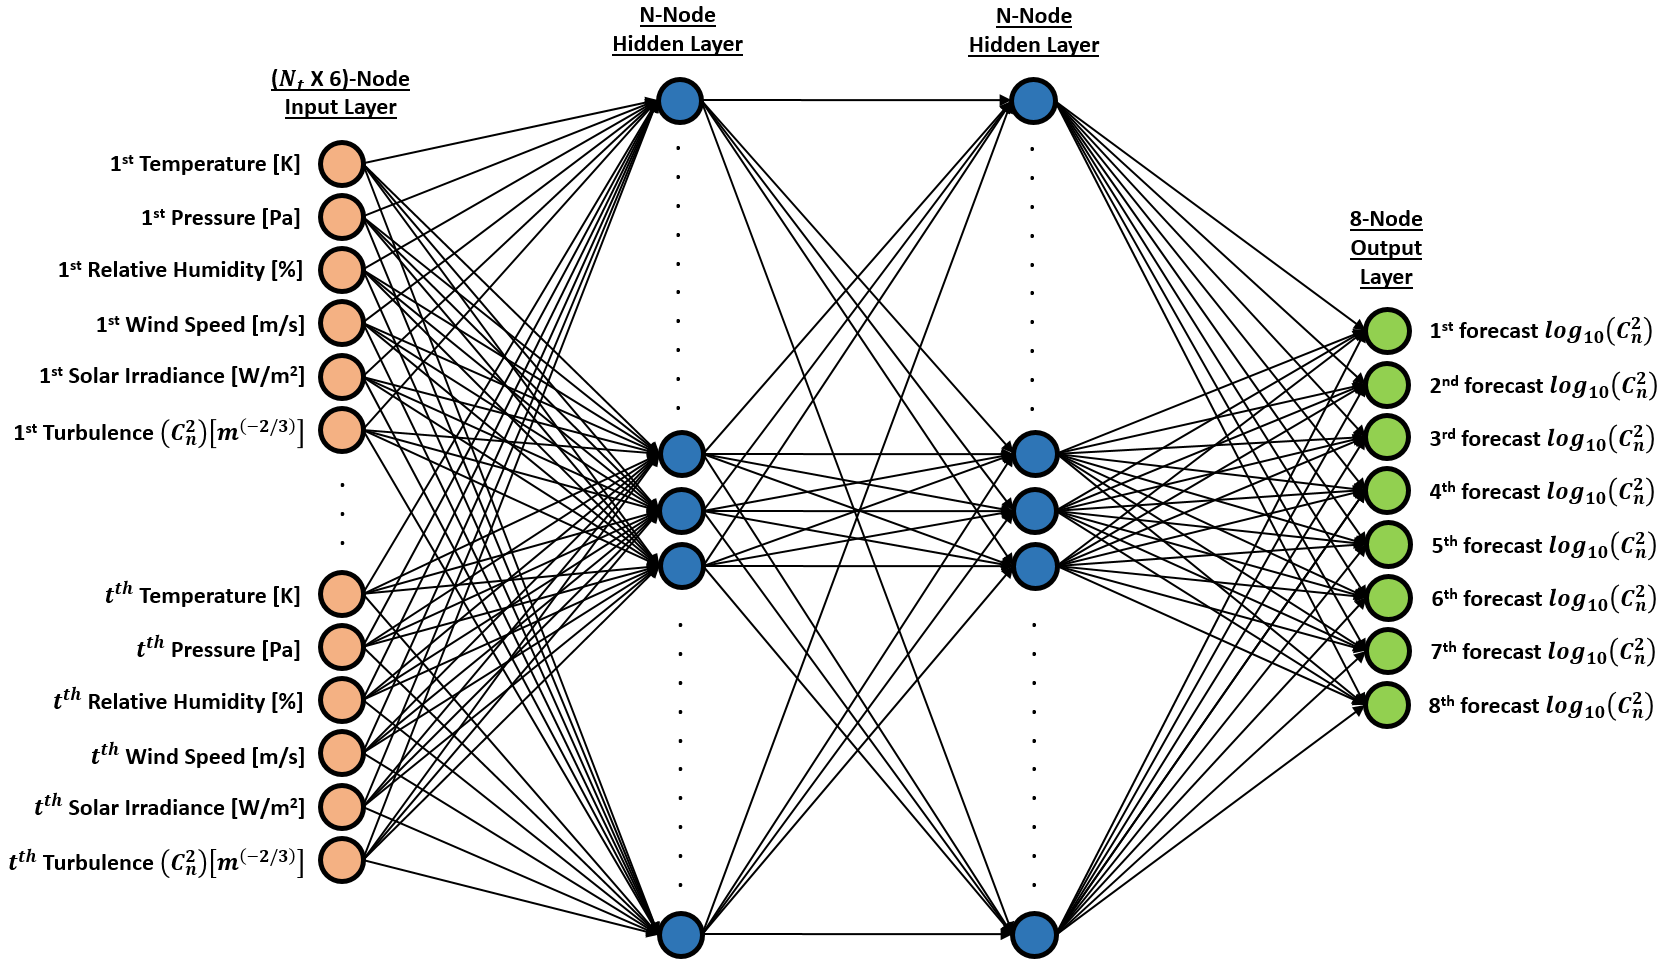
\includegraphics[width=0.99\textwidth]
	{architecture_MLP_forecast.png}
	\hfill
	\caption{Multi-layer MLP architecture with multiple time steps of weather as inputs and eight forecasts of turbulence as outputs}
	\label{fig:architecture_MLP_forecast}
\end{figure}
The output is a layer of eight nodes whose activations are eight time steps of measured $log_{10}(C_{n}^{2})$ \emph{after} the last time step in the input layer. The first node is the first time step in the forecast, the second node the second time step, and so on until the eighth node which is the eighth time step in the forecast. The \ac{ReLU} activation function is applied to the nodes of each hidden layer, but not the output layer so the trained model is not bounded during inference.

The flattening of input variables at multiple time steps to a single layer in the \ac{MLP} removes all information about the temporal relationship between the nodes. The \ac{RNN} architecture, however, preserves the temporal relationship of the model inputs as described above. Figure \ref{fig:architecture_RNN_single_layer_unrolled_to_outputs} illustrates a single-layer \ac{RNN} architecture and how its final hidden state $h_{t}$ is processed to predict the eight $log_{10}(C_{n}^{2})$ forecasts.
\begin{figure}[h!]
	\centering
	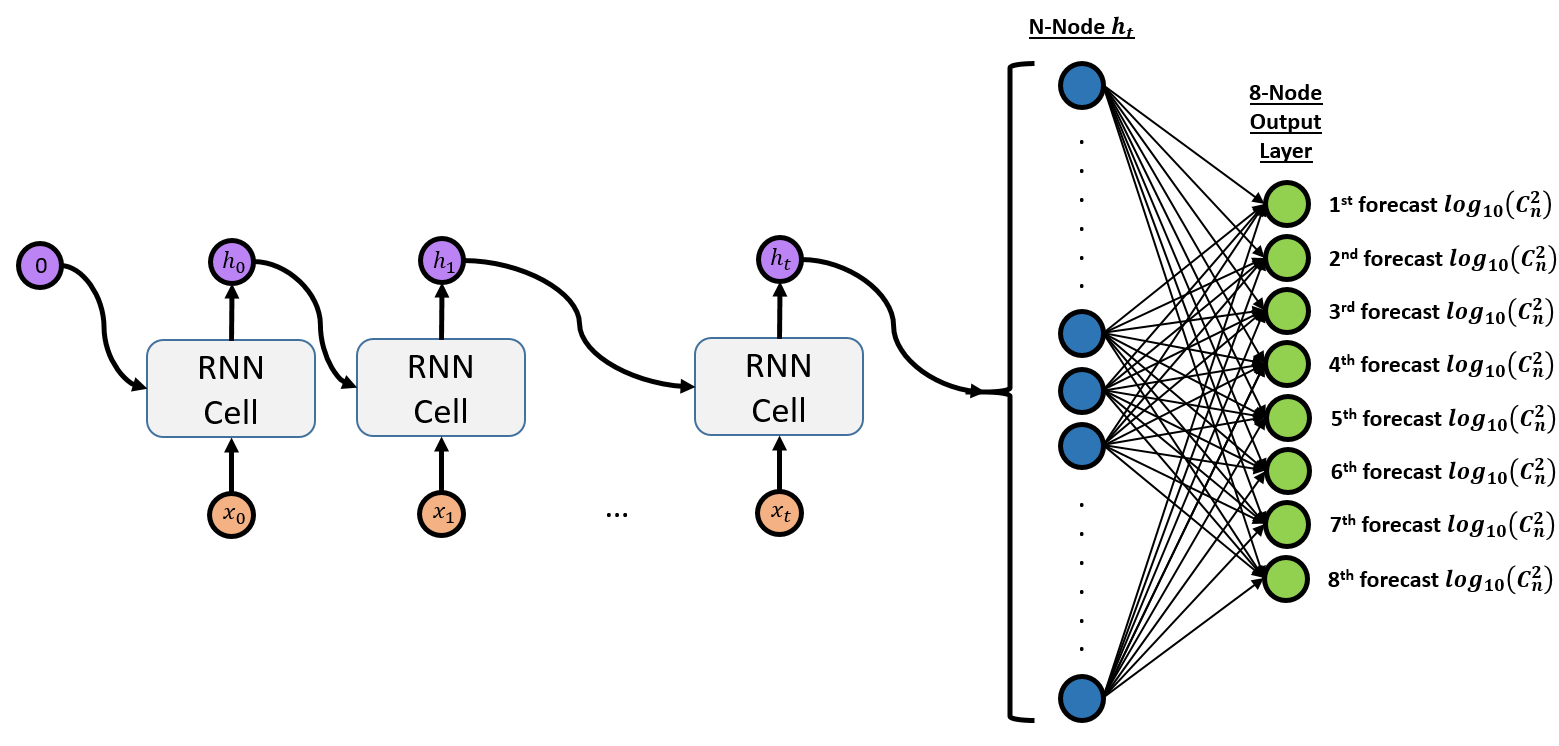
\includegraphics[width=0.99\textwidth]
	{architecture_RNN_single_layer_unrolled_to_outputs.png}
	\hfill
	\caption{Single-layer RNN architecture with multiple time steps of weather as inputs and eight forecasts of turbulence as outputs}
	\label{fig:architecture_RNN_single_layer_unrolled_to_outputs}
\end{figure}
The input $x_{t}$ is combined with the previous hidden state $h_{t-1}$ to update the current hidden state $h_{t}$ according to the type of \ac{RNN} cell employed. The final hidden state is simply a single layer of N-nodes and is fully-connected to the eight nodes in the output layer like in the \ac{MLP}. Throughout this manuscript, Figure \ref{fig:architecture_RNN_single_layer_unrolled_to_outputs} illustrates the exact architecture of an \ac{RNN} model with a single hidden layer. Figure \ref{fig:architecture_RNN_multi_layer_unrolled_to_outputs} illustrates the exact architecture when two hidden \ac{RNN} layers are employed.
\begin{figure}[h!]
	\centering
	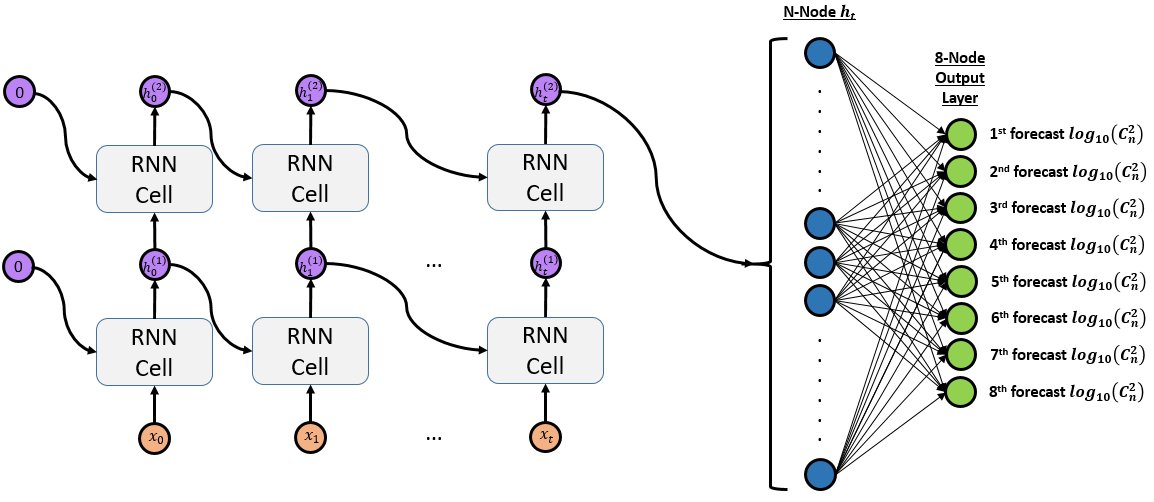
\includegraphics[width=0.99\textwidth]
	{architecture_RNN_multi_layer_unrolled_to_outputs.png}
	\hfill
	\caption{Multi-layer RNN architecture with multiple time steps of weather as inputs and eight forecasts of turbulence as outputs}
	\label{fig:architecture_RNN_multi_layer_unrolled_to_outputs}
\end{figure}
Note that in Figures \ref{fig:architecture_RNN_single_layer_unrolled_to_outputs} and \ref{fig:architecture_RNN_multi_layer_unrolled_to_outputs} the initial hidden state in the entire process is 0 (zero) as illustrated by the purple nodes on the far left of each Figure. This is the default behavior in PyTorch \cite{PyTorch} and is used throughout this work. The \ac{RNN} updating of the hidden state is considered to be a ``warming up" process to make a prediction at the end. In the application of the \ac{RNN} architectures presented here, $x_{t} = \left(\text{temp}, \text{press}, \text{rh}, \text{wind spd}, \text{solar irr}, log_{10}(C_{n}^{2})\right)_{t}$.

\section{Optimization and the Loss Function}
There are two steps in training a model. First is forward propagation in which the network makes a prediction by passing input values through the architecture and applying the learned parameters (weights and biases). The second step is backward propagation where the network adjusts its parameters according to their gradients (derivatives) with respect to the loss. The adjustment of the parameters is done by an optimization algorithm, the most common being gradient descent. Gradient descent is an algorithm used to find the values of the model parameters that minimizes the loss function (also called the cost function).

Gradient descent starts with an initial value such as 0 (zero) or a small random value. Next, the loss (cost) is calculated between model output and truth using a loss function such as \ac{MSE} in
\begin{equation} \label{eq:MSE}
	\text{MSE} = \frac{1}{N} \sum_{n=1}^{N} \left(x_{n} - y_{n}\right)^{2},
\end{equation}
where $x$ is model output and $y$ is truth. \ac{MSE} is a popular loss function in regression models and is used exclusively in this work for model training. The gradient (first partial derivative) of the loss with respect to each model parameter (weights and biases) is calculated and it indicates the direction and magnitude of greatest \emph{ascent} of the loss function. Since the algorithm is trying to minimize the loss function, the negative gradient (hence gradient \emph{descent}) is employed. One modeling hyperparameter is the \emph{learning rate} which scales the size of the adjustment to the parameters. Figure \ref{fig:gradient_descent_trivial} \cite{gradient_descent_trivial} illustrates a very simple example of gradient descent of the loss function with respect to a single parameter, weight $w$.
\begin{figure}[h!]
	\centering
	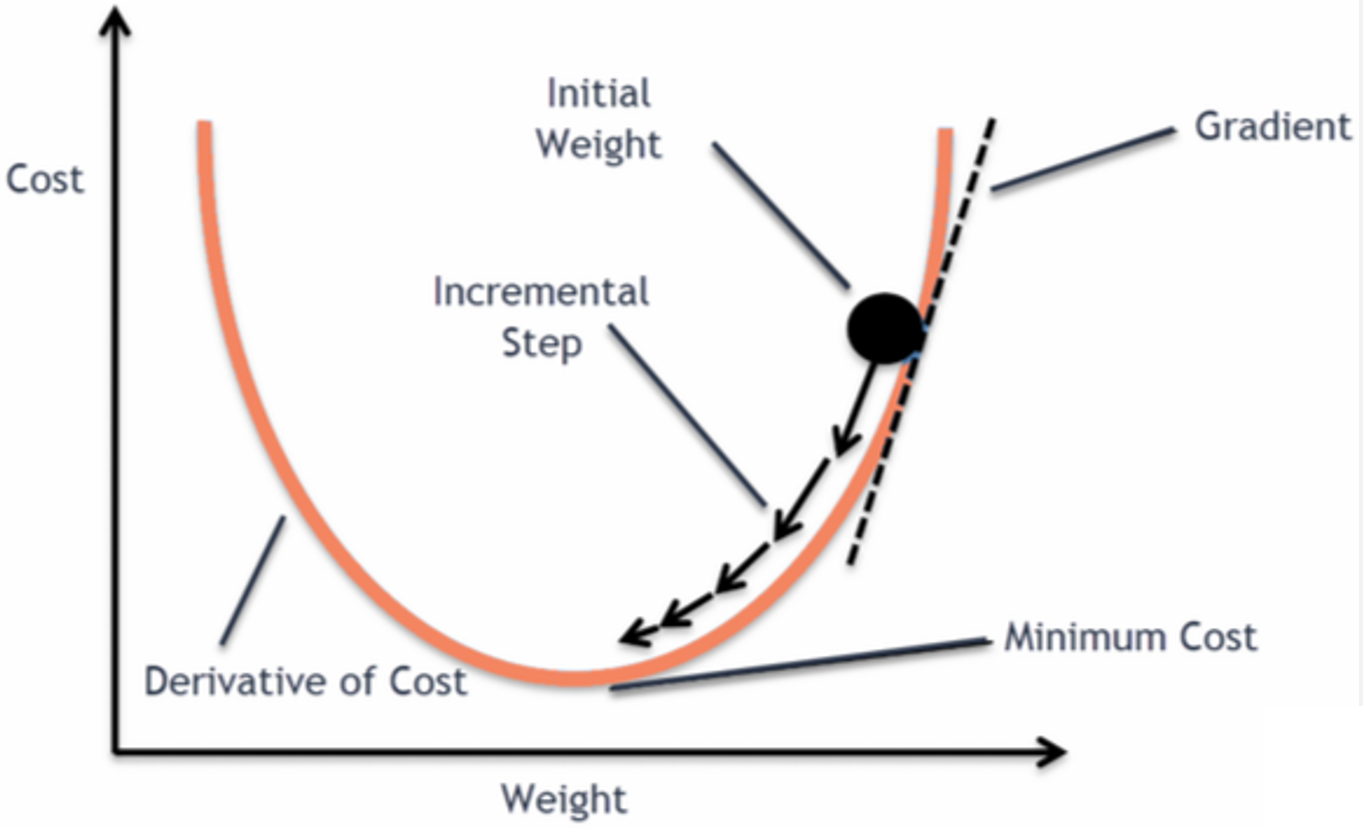
\includegraphics[width=0.7\textwidth]
	{gradient_descent_simple.png}
	\hfill
	\caption{Gradient descent of a trivial loss (cost) function}
	\label{fig:gradient_descent_trivial}
\end{figure}
The loss is plotted with respect to the weight's value where the orange curve is the derivative of the loss function with respect to the weight. The initial weight is shown at the top right of the derivative curve and the gradient is the dashed tangent line. As stated, the gradient is actually the direction and magnitude of steepest \emph{ascent} but the negative is used for steepest \emph{descent}. Multiple incremental steps of the weight's value is shown, each getting slightly smaller than the previous because the slope of the derivative curve is less steep as the minimum is reached. The learning rate hyperparameter proportionately adjusts the size of the incremental steps in Figure \ref{fig:gradient_descent_trivial}.

Figure \ref{fig:gradient_descent_trivial} illustrates a trivial example of gradient descent. In practice, the loss function with respect to model parameters is very complicated. A nontrivial case of gradient descent is in Figure \ref{fig:gradient_descent_nontrivial} \cite{gradient_descent_nontrivial}.
\begin{figure}[h!]
	\centering
	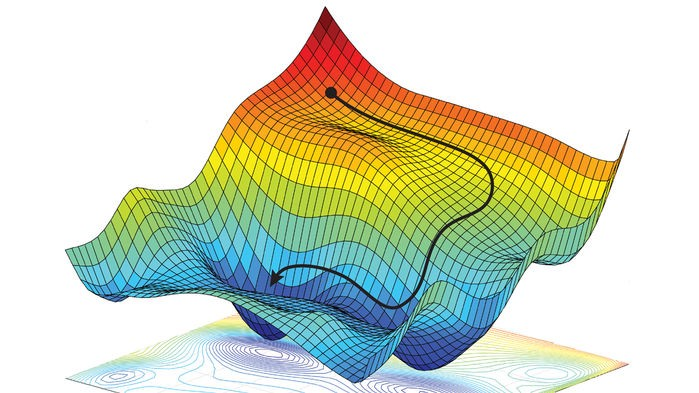
\includegraphics[width=0.7\textwidth]
	{gradient_descent_complex.png}
	\hfill
	\caption{Gradient descent of a nontrivial loss (cost) function}
	\label{fig:gradient_descent_nontrivial}
\end{figure}
An arrow illustrates how gradient descent moves through this map by starting at a high loss and iteratively stepping downhill until the global minimum is reached.

The derivative of the loss with respect to a parameter that directly calculates the output is simple to compute. The derivative of the loss with respect to a parameter near the front of the architecture, like in the first fully-connected layer of a 5-layer \ac{MLP}, is not so simple. The change in a parameter far away from the output causes a change in the parameters that are down the chain toward the output. To handle the train of changes, the chain rule is employed. PyTorch's automatic differentiation engine \textit{autograd} handles this entire process \cite{PyTorch}.

There are three common variations of gradient descent. \emph{Batch} gradient descent updates the model parameters based on the loss of the entire training set. So if the model is shown the training set 10 total times, then batch gradient descent provides 10 updates. \emph{Mini-batch} gradient descent updates the parameters every time a sub-sample of N training examples is shown to the model. In this work a mini-batch size of 32 is used exclusively. \emph{Stochastic} gradient descent updates the parameters after every training example. If a training set has 1 million examples and the entire set is only used once, then the model parameters will update 1 million times.

The optimization algorithm used explicitly in this work is \textit{AdamW} \cite{loshchilov2019decoupled} which is a variant of the originally proposed \textit{Adam} \cite{kingma2017adam}. The name \textit{Adam} is derived from adaptive moment estimation because it computes individual adaptive learning rates for different parameters from estimates of first and second moments of the gradients. Adaptive gradient methods have become the default method of choice for training feed-forward and recurrent neural networks. The variant AdamW modifies the original Adam to correctly apply weight decay regularization. The modification substantially improves Adam's generalization on image classification datasets of which it previously performed worse. The improved generalization motivates the use of AdamW in this work.

\section{Chapter Summary}
The chapter has laid the foundation of machine learning modeling including the very basics of training and testing, the fundamental \ac{MLP} and \ac{RNN} architectures and how they apply to turbulence modeling, popular variants of the \ac{RNN} cells, and the algorithm for parameter optimization.